\documentclass[11pt]{article}

\usepackage[margin=1in]{geometry}
\usepackage[T1]{fontenc}
\usepackage{lmodern}
\usepackage{microtype}
\usepackage{amsmath,amssymb}
\usepackage[dvipsnames]{xcolor}
\usepackage{enumitem}
\usepackage{needspace}
\usepackage[most]{tcolorbox}
\usepackage{tikz}
\usepackage[hidelinks]{hyperref}

\hypersetup{
  pdftitle={Homework 3, MATH 327, Fall 2026},
  pdfauthor={Manish Patnaik},
  pdfsubject={MATH 327 homework problems}
}

\definecolor{courseblue}{HTML}{1F4E79}
\definecolor{lightblue}{HTML}{EAF2F8}
\definecolor{boxborder}{HTML}{B8CBDC}
\definecolor{darkgray}{HTML}{333333}

\setlength{\parindent}{0pt}
\setlength{\parskip}{0.55em}
\setlist[enumerate]{leftmargin=2em, itemsep=0.25em, topsep=0.3em}

\newtcolorbox{exercise}[2][]{
  enhanced,
  colback=white,
  colframe=boxborder,
  colbacktitle=lightblue,
  coltitle=courseblue,
  fonttitle=\bfseries,
  title={Exercise #2},
  boxrule=0.6pt,
  arc=1mm,
  left=2.5mm,
  right=2.5mm,
  top=1.5mm,
  bottom=1.5mm,
  before skip=0.8em,
  after skip=0.8em,
  #1
}

% Diagram modes: 1 = short diagonals, 2 = long diagonals, 3 = all.
\newcommand{\hexagondiagonals}[1]{%
  \begin{tikzpicture}[scale=0.85]
    \foreach \i in {1,...,6} {
      \pgfmathsetmacro{\vertexangle}{60*(\i-1)}
      \coordinate (v\i) at (\vertexangle:1.65);
      \node at (\vertexangle:2.05) {$v_{\i}$};
    }
    \draw[gray] (v1) -- (v2) -- (v3) -- (v4) -- (v5) -- (v6) -- cycle;
    \ifnum#1=2\relax\else
      \foreach \i in {1,...,6} {
        \pgfmathtruncatemacro{\j}{mod(\i+1,6)+1}
        \draw[thick,courseblue] (v\i) -- (v\j);
      }
    \fi
    \ifnum#1=1\relax\else
      \foreach \i in {1,...,3} {
        \pgfmathtruncatemacro{\j}{\i+3}
        \draw[thick,BurntOrange] (v\i) -- (v\j);
      }
    \fi
    \ifnum#1=2\relax\else
      \foreach \i in {1,...,6} {
        \pgfmathsetmacro{\labelangle}{60*\i}
        \node[fill=white,inner sep=1pt,font=\scriptsize,text=courseblue]
          at (\labelangle:0.825) {$d_{\i}$};
      }
    \fi
    \ifnum#1=1\relax\else
      \foreach \i in {1,...,3} {
        \pgfmathsetmacro{\labelangle}{60*(\i-1)}
        \node[fill=white,inner sep=1pt,font=\scriptsize,text=BurntOrange]
          at (\labelangle:1.2) {$\ell_{\i}$};
      }
    \fi
    \foreach \i in {1,...,6} {\fill (v\i) circle (2pt);}
  \end{tikzpicture}%
}

\newcommand{\chapterheading}[1]{%
  \par\vspace{0.5em}
  {\color{courseblue}\Large\bfseries #1}\par\vspace{0.35em}
  {\color{boxborder}\hrule height 0.6pt}\vspace{0.35em}
}

\newcommand{\sectionheading}[1]{%
  \Needspace{8\baselineskip}
  \vspace{0.25em}
  {\color{darkgray}\large\bfseries #1}\par
}

\begin{document}

\begin{center}
  \colorbox{lightblue}{%
    \begin{minipage}{0.92\textwidth}
      \vspace{0.6em}
      \begin{tabular*}{\textwidth}{@{\extracolsep{\fill}}lr}
        {\color{courseblue}\bfseries\LARGE Homework 3} &
        {\color{courseblue}\bfseries\LARGE MATH 327}\\[0.4em]
        \multicolumn{2}{l}{\color{darkgray}\bfseries Fall 2026}\\[0.35em]
        \multicolumn{2}{l}{\color{darkgray}Covers Lectures 15--19}\\[0.2em]
        \multicolumn{2}{l}{\color{darkgray}Suggested completion date: Monday, October 26}
      \end{tabular*}
      \vspace{0.5em}
    \end{minipage}}
\end{center}

\vspace{0.5em}

Unless otherwise indicated, the following exercises are from Michael Artin's
\emph{Algebra}, second edition.

\chapterheading{Chapter 2: Groups}

\sectionheading{Section 10: The Correspondence Theorem}

\begin{exercise}{10.5 (Adapted)}
Let $\varphi\colon S_4\to S_3$ be the homomorphism described in
Example 2.5.13. In class we determined the subgroups
\[
  A=\varphi^{-1}\bigl(\langle(123)\rangle\bigr)
  \qquad\text{and}\qquad
  H_1=\varphi^{-1}\bigl(\langle(13)\rangle\bigr).
\]
Perform a similar analysis to determine the subgroup
\[
  H_2=\varphi^{-1}\bigl(\langle(12)\rangle\bigr).
\]
\textit{Hint.} Relabel the vertices of the square as shown below and
consider its geometric symmetries as permutations in $S_4$.
\begin{center}
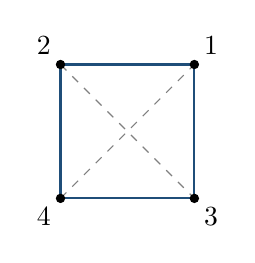
\begin{tikzpicture}[scale=0.85]
  \draw[thick,courseblue] (0,0) -- (2,0) -- (2,2) -- (0,2) -- cycle;
  \draw[dashed,gray] (0,0) -- (2,2) (0,2) -- (2,0);
  \fill (2,2) circle (2pt) node[above right] {$1$};
  \fill (0,2) circle (2pt) node[above left] {$2$};
  \fill (0,0) circle (2pt) node[below left] {$4$};
  \fill (2,0) circle (2pt) node[below right] {$3$};
\end{tikzpicture}
\end{center}
\end{exercise}

\begin{exercise}{S.1 (Supplementary)}
Prove that there is no surjective homomorphism $S_5\to S_4$.
\end{exercise}

\sectionheading{Dihedral Groups and Group Actions}

\begin{exercise}{1 (Supplementary)}
Let $n\geq3$. Define $D_{2n}$ by the presentation
\[
  D_{2n}=\langle x,y\mid x^n=1,\ y^2=1,\ yx=x^{n-1}y\rangle.
\]

\begin{enumerate}[label=\textbf{(\alph*)}]
	\item Prove that every element of $D_{2n}$ can be written uniquely in one of
	the forms
	\[
	x^k \qquad\text{or}\qquad x^k y,
	\qquad 0\leq k<n.
	\] Conclude that $D_{2n}$ has exactly $2n$ elements.

	\item Let $H:=\{1,x,\ldots,x^{n-1}\}$. Show that $H$ is a normal subgroup of $D_{2n}$.

	\item Let $I:=\{1,y\}$. Is $I$ normal in $D_{2n}$? Justify your answer.


	\end{enumerate}


\end{exercise}

\begin{exercise}{2 (Supplementary)}
Let a group $G$ act on a set $S$. Recall that the \emph{orbit} of
$s\in S$ and its \emph{stabilizer} are defined by
\[
  O_s:=\{g\circ s\mid g\in G\},
  \qquad
  \operatorname{Stab}_G(s):=\{g\in G\mid g\circ s=s\}.
\]
Consider the natural action of $D_8$, the symmetry group of the square,
on its vertices $V=\{v_1,v_2,v_3,v_4\}$, labeled as follows.
\begin{center}
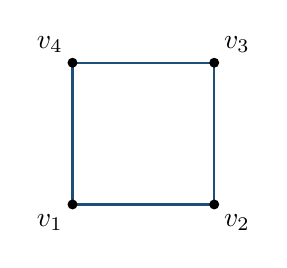
\begin{tikzpicture}[scale=0.9]
  \draw[thick,courseblue] (0,0) -- (2,0) -- (2,2) -- (0,2) -- cycle;
  \fill (0,0) circle (2pt) node[below left] {$v_1$};
  \fill (2,0) circle (2pt) node[below right] {$v_2$};
  \fill (2,2) circle (2pt) node[above right] {$v_3$};
  \fill (0,2) circle (2pt) node[above left] {$v_4$};
\end{tikzpicture}
\end{center}
Determine the orbit $O_{v_1}$ and the stabilizer
$\operatorname{Stab}_{D_8}(v_1)$.
\end{exercise}

\begin{exercise}[breakable]{3 (Supplementary)}
Consider the natural action of $D_{12}$ on the vertices
$V=\{v_1,\ldots,v_6\}$ of a regular hexagon, labeled counterclockwise
as shown below. Let $x$ be counterclockwise rotation through $\pi/3$,
and let $y$ be reflection across the diagonal joining $v_1$ and $v_4$.
\begin{center}
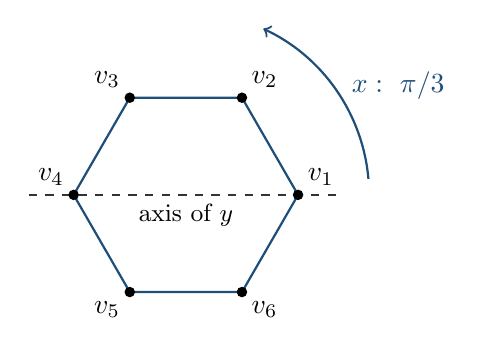
\begin{tikzpicture}[scale=0.95]
  \draw[thick,courseblue]
    (0:1.5) -- (60:1.5) -- (120:1.5) -- (180:1.5)
    -- (240:1.5) -- (300:1.5) -- cycle;
  \draw[dashed,thick,darkgray] (-2.1,0) -- (2.1,0);
  \node[below,font=\small] at (0,0) {axis of $y$};
  \fill (0:1.5) circle (2pt) node[above right] {$v_1$};
  \fill (60:1.5) circle (2pt) node[above right] {$v_2$};
  \fill (120:1.5) circle (2pt) node[above left] {$v_3$};
  \fill (180:1.5) circle (2pt) node[above left] {$v_4$};
  \fill (240:1.5) circle (2pt) node[below left] {$v_5$};
  \fill (300:1.5) circle (2pt) node[below right] {$v_6$};
  \draw[->,thick,courseblue] (5:2.45) arc (5:65:2.45);
  \node[right,text=courseblue] at (35:2.55) {$x:\ \pi/3$};
\end{tikzpicture}
\end{center}
\begin{enumerate}[label=\textbf{(\alph*)}]
  \item Describe geometrically each of the transformations
        $xy$, $x^2y$, $x^3y$, $x^4y$, and $x^5y$.
        Identify the axis of any reflection that occurs.
        Here products act from right to left, so $xy$ means first
        apply $y$, then $x$.
  \item Describe the homomorphism $\rho\colon D_{12}\to S_6$
        induced by this action by writing $\rho(x)$ and $\rho(y)$
        in cycle notation. Determine $\ker\rho$.
  \item \textbf{Short diagonals.}
        Let $\mathcal D_s=\{d_1,\ldots,d_6\}$, where
        $d_i=\overline{v_i v_{i+2}}$ and vertex subscripts are read
        modulo $6$.
        A diagonal is an unordered pair of endpoints, so a symmetry
        may preserve a diagonal while exchanging its endpoints.
        The short diagonals are shown in blue below.
        \begin{center}
          \hexagondiagonals{1}
        \end{center}
        Determine the orbits of $D_{12}$ on $\mathcal D_s$ and compute
        $\operatorname{Stab}_{D_{12}}(d_1)$.
        Describe the induced homomorphism
        $\rho_s\colon D_{12}\to S_6$ by giving $\rho_s(x)$ and
        $\rho_s(y)$ in cycle notation, using $d_i\leftrightarrow i$.
        Determine $\ker\rho_s$.
  \item \textbf{Long diagonals.}
        Let $\mathcal D_\ell=\{\ell_1,\ell_2,\ell_3\}$, where
        $\ell_i=\overline{v_i v_{i+3}}$.
        These diagonals join opposite vertices and are shown in orange.
        \begin{center}
          \hexagondiagonals{2}
        \end{center}
        Determine the orbits of $D_{12}$ on $\mathcal D_\ell$ and
        compute $\operatorname{Stab}_{D_{12}}(\ell_1)$.
        Describe the induced homomorphism
        $\rho_\ell\colon D_{12}\to S_3$ by giving $\rho_\ell(x)$ and
        $\rho_\ell(y)$ in cycle notation, using $\ell_i\leftrightarrow i$.
        Determine $\ker\rho_\ell$.
  \item \textbf{All diagonals.}
        Let $\mathcal D=\mathcal D_s\cup\mathcal D_\ell$ be the set of
        all nine diagonals, shown below.
        \begin{center}
          \hexagondiagonals{3}
        \end{center}
        Determine the orbits of $D_{12}$ on $\mathcal D$ and compute
        the stabilizer of a representative from each orbit.
        Describe the induced homomorphism
        $\rho_{\mathcal D}\colon D_{12}\to S_9$ by giving the images
        of $x$ and $y$ in cycle notation, using
        \[
          (d_1,d_2,d_3,d_4,d_5,d_6,\ell_1,\ell_2,\ell_3)
          \longleftrightarrow (1,2,3,4,5,6,7,8,9).
        \]
        Determine $\ker\rho_{\mathcal D}$.
\end{enumerate}
\end{exercise}

\sectionheading{Section 11: Product Groups}

\begin{exercise}{11.6}
Let $G$ be a group that contains normal subgroups of orders $3$ and $5$,
respectively. Prove that $G$ contains an element of order $15$.
\end{exercise}

\begin{exercise}{11.9}
Let $H$ and $K$ be subgroups of a group $G$. Prove that the product set
$HK$ is a subgroup of $G$ if and only if $HK=KH$.
\end{exercise}


\sectionheading{Section 12: Quotient Groups}

\begin{exercise}{12.4}
Let $H=\{\pm1,\pm i\}$ be the subgroup of $G=\mathbb{C}^{\times}$ of
fourth roots of unity. Describe the cosets of $H$ in $G$ explicitly.
Is $G/H$ isomorphic to $G$?
\end{exercise}

\begin{exercise}{12.5}
Let $G$ be the group of upper triangular real matrices
$\begin{bmatrix}a&b\\0&d\end{bmatrix}$ with $a$ and $d$ different from
zero. For each of the following subsets, determine whether or not $S$ is
a subgroup, and whether or not $S$ is a normal subgroup. If $S$ is a
normal subgroup, identify the quotient group $G/S$.
\begin{enumerate}[label=\textbf{(\roman*)}]
  \item $S$ is the subset defined by $b=0$.
  \item $S$ is the subset defined by $d=1$.
  \item $S$ is the subset defined by $a=d$.
\end{enumerate}
\end{exercise}

\vfill
{\small\color{darkgray}Compiled \today.}

\end{document}
